\documentclass[xcolor=dvipsnames,aspectratio=169,t]{beamer}
  % t means frames are vertically centered to the top
\usepackage{slides-header}
\title{Systems of Linear Equations}

\begin{document}
\maketitle

\begin{frame}{Linear Equations}

  A \alert{linear equation} of $x_1, \dots, x_n$ is an equation that can be written in the form
  \[ a_1x_1 + a_2x_2 + \ldots + a_nx_n = b \]
  where
  \bi
  \ii $b$ and the \colorb{coefficients} $a_1, a_2, \ldots , a_n$ are constants (real numbers), and
  \ii we have $n$ \colorb{variables} denoted $x_1, x_2, \ldots , x_n$. 
  \ei
  
  \pause
  \begin{example}
    Determine whether the equation is \alert{linear} in $x_1$, $x_2$, and $x_3$.
    \medskip
    
    \begin{tasks}(2)
      \task $\dsty  \cos{ \left( \frac{\pi}{3} \right)} x_1 + e^4 x_2 -  \frac{x_3}{\pi} = -5$
      \task $\dsty  3x_1 + 2x_1x_2 - 3x_3 = 8$
      \bigskip
      \task $\dsty  2 x_1 +  4 \sqrt{x_2} - 3x_3 = 8$
    \end{tasks}
  \end{example}
   
  \end{frame}


\begin{frame}{Systems of Linear Equations}
  A \alert{system of linear equations} is a collection of one or more linear equations involving the same variables $x_1, \ldots x_n$.
  \medskip
  
  \begin{columns}[T]
    \column{0.5\tw}
      \colorb{
      A system of two linear equations with two variables, $x_1$ and $x_2$. 
      \begin{align*}
        2x_1 -9x_2 &=12 \\
        4x_1 +2x_2 &=-16
      \end{align*}
      }
    
    \column{0.5\tw}
      \alert{A system of three linear equations with four variables, $x_1, x_2, x_3$, and $x_4$.
      \onslide*<1>{
      \begin{align*}
        & 8x_1+7x_2-x_3 - 5x_4 = 10 \\
        & 2x_1-6x_2- 12x_4 = 0 \\
        & 0.5x_1-0.01x_2+2.1x_3 - 1.5x_4 = -2 \\
      \end{align*}
      }%
      \onslide*<2->{
      \[
      \begin{array}{rrrrrr}
        8x_1 & +7x_2 & -x_3 & - 5x_4 & = & 10 \\
        2x_1 & -6x_2 &      & - 12x_4 & = & 0 \\
        0.5x_1 & -0.01x_2 & +2.1x_3 & - 1.5x_4 & = & -2 \\
      \end{array}
      \]
      }
      }
  \end{columns}
  \vspace*{3em}
  
  \onslide<3->{
  We frequently refer to a system of linear equations as a \alert{linear system}.
  }
\end{frame}

\begin{frame}{Visualizing the Solution}

  A \alert{solution} to a linear system is an ordered list of numbers $(s_1, s_2, \ldots s_n)$ that make \alert{all} of the equations in the system true when we substitute $x_1 = s_1, \ldots , x_n=s_n$.
  \bigskip
  
  \begin{columns}[T]
    \column{0.25\tw}
    For example, $(x_1,x_2)=(-3,-2)$ is a solution to the system
    \begin{align*}
      & \colorb{2x_1 -9x_2 = 12 }\\
      & \colorr{4x_1 +2x_2 =-16 }
    \end{align*}
   
    \column{0.75\tw}
    \vspace*{-1em}
    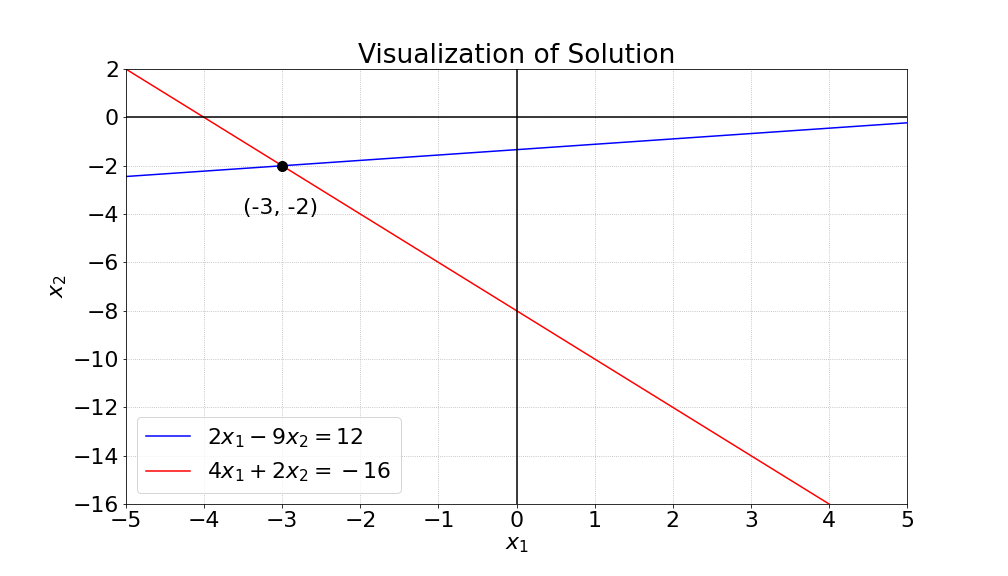
\includegraphics[width=0.925\tw]{images/fig-two-lines1.png}
  \end{columns}

\end{frame}


\begin{frame}{Review: Solving a Linear System}

  {\small
  You probably already have some strategies for solving some systems of equations. For example:
  \begin{align*}
    & 2x_1 -9x_2 =12 \\
    & 4x_1 +2x_2=-16
  \end{align*} }
  \pause
  
  \vspace{-0.25in}
   
  \begin{columns}[T]

    \column{0.5\tw}
            {\small
              \bb
     \ii Multiply top equation by $-2$ and add to bottom equation.

     \vspace{-0.25in}
   \begin{align*}
      & 2x _1- 9x_2 =12 \\
       & 0x_1 + 20x_2=-40
   \end{align*}

  \ii Divide bottom equation by 20.

     \vspace{-0.25in}
   \begin{align*}
      & 2x_1 -  9x_2 =12 \\
       & 0x_1 + x_2=-2
   \end{align*}
   \ee }
   
     \column{0.5\tw}

     {\small
   \bb
     \addtocounter{enumi}{2}
   \ii Add 9 times bottom equation to top equation:

     \vspace{-0.25in}
\begin{align*}
  & 2x_1 +0x_2 =-6 \\
      & 0x_1 + x_2 =-2
\end{align*}

   \ii Divide top equation by 2:

     \vspace{-0.25in}
\begin{align*}
     & x_1  =-3 \\
      & x_2 =-2
\end{align*}

\ee }

\end{columns}

\end{frame}


\begin{frame}{How Many Solutions Exist?}
  \pause

  \vspace{-1em}
  
  \begin{columns}[b]
    \column{0.5\tw}
      {\small
      \begin{align*}
        & \colorr{2x_1+4x_2=10} \\
        & \colorb{4x_1+8x_2 = 10}
      \end{align*} }
      
      \vspace{-0.3in}
      
      \quad 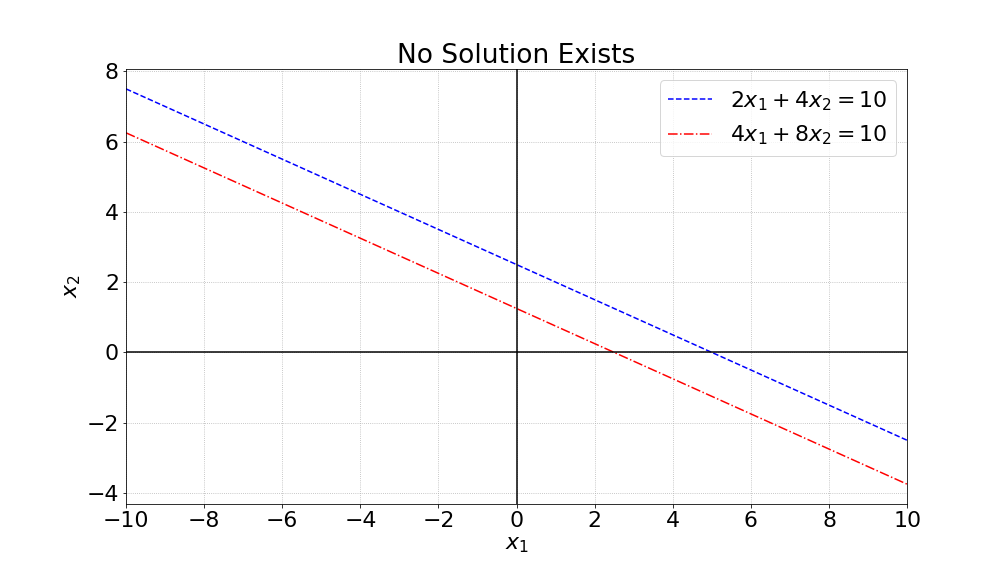
\includegraphics[width=0.8\tw]{images/fig-two-lines3.png}
    
    \column{0.5\tw}
      {\small
      \begin{align*}
        & \colorr{2x_1+4x_2=10} \\
        & \colorb{4x_1+8x_2 = 20}
      \end{align*} }
      
      \vspace{-0.3in}
      
      \quad 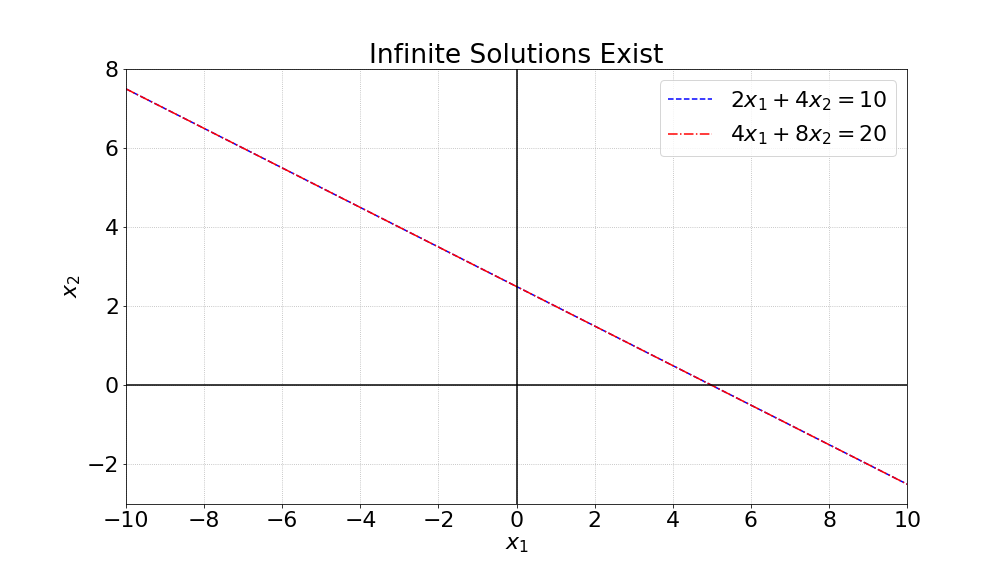
\includegraphics[width=0.8\tw]{images/fig-two-lines2.png}
  \end{columns}
  
  \pause
  A system of linear equations may have:
  \begin{itemize}
  \item \colorb{No solution.} Such systems are called \alert{inconsistent}, or
  \item Solutions (called \alert{consistent}).  How many solutions?
    \begin{itemize}
      \item \colorb{Exactly one solution.}
      \item \colorb{Infinitely many solutions.}
    \end{itemize}
  \end{itemize}
\end{frame}


\begin{frame}{Matrix Notation}

  \bi
  \ii Good news: There is a systemic way to solve a linear system (if a solution exists).
  \ii Bad news: It can involve many algebraic steps.
  \ii We can use a rectangular array called a \alert{matrix} to help organize the work.
  \ei

  \vspace*{2em}
  
  \begin{columns}[T]
    \column{0.33\tw}
    System of linear equations:
    \begin{align*}
      & \alert{2}x_1 \alert{-9}x_2 = \colorb{12} \\
      & \alert{4}x_1 +\alert{2}x_2= \colorb{-16}
    \end{align*} 

    \column{0.33\tw}
    The \alert{coefficient matrix}:
      \[ 
        \begin{bmatrix}
          \alert{2} & \alert{-9} \\
          \alert{4} & \alert{2} 
        \end{bmatrix}
      \]

    \column{0.33\tw}
    The \alert{augmented matrix}:
      \[ 
        \begin{bmatrix}
          \alert{2} & \alert{-9} & \colorb{12}\\
          \alert{4} & \alert{2} & \colorb{-16}
        \end{bmatrix}
      \]
  \end{columns}

\end{frame}

\begin{frame}{Example}

  \begin{example}
  Give the augmented matrix for the system of linear equations.
    \begin{align*}
      & 8x_1+7x_2-x_3 - 5x_4 = 10 \\
      & 2x_1-6x_2- 12x_4 = 0 \\
      & 0.5x_1-0.01x_2+2.1x_3 - 1.5x_4 = -2 \\
    \end{align*}
  \end{example}

  \pause
  \begin{solution}
    \[ \begin{bmatrix}
      8 & 7 & -1 & -5 & 10 \\
      2 & -6 & 0 & -12 & 0 \\
      0.5 & -0.01 & 2.1 & -1.5 & -2
    \end{bmatrix} \]
  \end{solution}
  
\end{frame}

\begin{frame}{Describing the Size of a Matrix}

  How many rows does the augmented matrix have? How many columns?
  
\[ \begin{bmatrix}
      8 & 7 & -1 & -5 & 10 \\
      2 & -6 & 0 & -12 & 0 \\
      0.5 & -0.01 & 2.1 & -1.5 & -2
    \end{bmatrix} \]

  \bi
  \ii \colorb{The augmented matrix above has 3 rows.} This means the system consists of 3 equations.
  \ii \colorr{The augmented matrix above has 5 columns}. This means there are 4 variables.
  \ei
  \bigskip

  Thus the augmented matrix above is a $\colorb{3} \times \colorr{5}$ (read as ``3 by 5'') matrix.

  \vspace*{1em}

  \pause
  \bbox
  \alert{Caution!} The order matters when describing the size of a matrix. 
  
  \phantom{Caution!} Always \alert{rows first}, then columns second!
  \ebox

\end{frame}

\begin{frame}{Solving a Linear System Using Matrices}

  {\small  Solve the following system.}
  {\small
   \[
   \begin{array}{l}
     2x_1 -9x_2 =12 \\
      4x_1 +2x_2=-16
  \end{array} \rightarrow
      \begin{bmatrix}
     2 & -9 & 12\\
     4 & 2 & -16
   \end{bmatrix} \]
   }

  %\vspace{-0.25in}
  
  \pause
  \begin{columns}[T]

     \column{0.5\tw}
            {\small
              \bb
     \ii Multiply top equation by $-2$ and add to bottom equation.

 %    \vspace{-0.25in}
\[  \begin{bmatrix}
     2 & -9 & 12\\
     0 & 20 & -40
   \end{bmatrix} \]

  \ii Divide bottom equation by 20.

 %    \vspace{-0.25in}
\[  \begin{bmatrix}
     2 & -9 & 12\\
     0 & 1 & -2
   \end{bmatrix} \]
\ee            }
   
     \column{0.5\tw}

     {\small
   \bb
     \addtocounter{enumi}{2}
   \ii Add 9 times bottom equation to top equation:

  % \vspace{-0.05in}
   \[  \begin{bmatrix}
     2 & 0 & -6 \\
     0 & 1 & -2
   \end{bmatrix} \]
 
   \ii Divide top equation by 2:

%   \vspace{-0.25in}
     \[  \begin{bmatrix}
     1 & 0 & -3 \\
     0 & 1 & -2
   \end{bmatrix} \]

\colorb{Thus, the solution is $(x_1,x_2) = (-3,-2)$.}
     
\ee }

\end{columns}

\end{frame}

\begin{frame}{Going One Dimension Up}

  {\small  Solve the following system.}
  
  {\small
   \[
   \begin{array}{l}
     x_1 +x_2 +x_3=7 \\
     x_1 -x_2 +2x_3= 7\\
     5x_1+x_2+x_3=11
  \end{array}  \pause \sim
      \begin{bmatrix}
        1 & 1 & 1 & 7\\
        1 & -1 & 2 & 7\\
        5 & 1 & 1 & 11
      \end{bmatrix}
      \rightarrow
       \begin{bmatrix}
        1 & 1 & 1 & 7\\
        0 & -2 & 1 & 0\\
        5 & 1 & 1 & 11
      \end{bmatrix}
    \rightarrow      \]
   }

  {\small
  \[    \rightarrow 
  \begin{bmatrix}
        1 & 1 & 1 & 7\\
        0 & -2 & 1 & 0\\
        0 & -4 & -4 & -24
      \end{bmatrix}
  \rightarrow
  \begin{bmatrix}
        1 & 1 & 1 & 7\\
        0 & -2 & 1 & 0\\
        0 & 0 & -6 & -24
  \end{bmatrix}
  \rightarrow
  \begin{bmatrix}
        1 & 1 & 1 & 7\\
        0 & -2 & 1 & 0\\
        0 & 0 & 1 & 4
      \end{bmatrix}  
  \rightarrow
  \begin{bmatrix}
        1 & 1 & 1 & 7\\
        0 & -2 & 0 & -4\\
        0 & 0 & 1 & 4
      \end{bmatrix}  
  \rightarrow
  \]}

  {\small
    \[ \rightarrow
  \begin{bmatrix}
        1 & 1 & 1 & 7\\
        0 & 1 & 0 & 2\\
        0 & 0 & 1 & 4
      \end{bmatrix}  
  \rightarrow
  \begin{bmatrix}
        1 & 0 & 1 & 5\\
        0 & 1 & 0 & 2\\
        0 & 0 & 1 & 4
      \end{bmatrix}  
  \rightarrow
  \begin{bmatrix}
        1 & 0 & 0 & 1\\
        0 & 1 & 0 & 2\\
        0 & 0 & 1 & 4
      \end{bmatrix}  
  \]}
    
\colorb{Thus $(x_1,x_2,x_3) = (1,2,4)$ is a solution of the linear system.}
  
\end{frame}

\begin{frame}{Elementary Row Operations}

  There are three operations we can apply to the rows of an augmented matrix:
  \bb
  \ii Change one row by \alert{adding a multiple of another row to it}.
  \ii \colorb{Swapping two rows}.
  \ii \colorg{Scaling one row} by multiplying all entries in the row by a \colorg{nonzero} constant.
  \ee

  \[
    \begin{bmatrix}
      1 & -8 & 0 & 6 \\
      0 & 0 & 2 & 8 \\
      0 & 1 & 0 & -3
    \end{bmatrix}
    \rightarrow 
    \begin{bmatrix}
      \colorr{1} & \colorr{0} & \colorr{0} & \colorr{-18} \\
      0 & 0 & 2 & 8 \\
      0 & 1 & 0 & -3
    \end{bmatrix}
    \rightarrow
    \begin{bmatrix}
      1 & 0 & 0 & -18 \\
      \colorb{0} & \colorb{1} & \colorb{0} & \colorb{-3} \\
      \colorb{0} & \colorb{0} & \colorb{2} & \colorb{8} 
    \end{bmatrix}
    \rightarrow
    \begin{bmatrix}
      1 & 0 & 0 & -18 \\
      0 & 1 & 0 & -3\\
      \colorg{0} & \colorg{0} & \colorg{1} & \colorg{4} 
    \end{bmatrix}
  \]
  \bigskip
 
  \pause
  \bbox
  Two matrices are \alert{row equivalent} if one matrix can be transformed into the other using elementary row operations.
  \ebox
 
\end{frame}
 
\begin{frame}{Equivalent Systems}

  \bi
\ii If the augmented matrices of two linear systems are \colorb{row equivalent}, then the two systems have the same solutions.
\colorb{
\[
    \begin{bmatrix}
        1 & 1 & 1 & 7\\
        1 & -1 & 2 & 7\\
        5 & 1 & 1 & 11
    \end{bmatrix}
    \mbox{ and } 
\begin{bmatrix}
        1 & 0 & 0 & 1\\
        0 & 1 & 0 & 2\\
        0 & 0 & 1 & 4
\end{bmatrix}
\mbox{ are row equivalent matrices!} \] }

  \ii If two linear systems have the same solutions, we say \alert{the two linear systems are equivalent}.
\alert{
\[    \begin{array}{l}
     x_1 +x_2 +x_3=7 \\
     x_1 -x_2 +2x_3= 7\\
     5x_1+x_2+x_3=11
\end{array}  \mbox{ and }
 \begin{array}{l}
     x_1 =1 \\
      x_2 = 2\\
     x_3 =4 
 \end{array} \mbox{ are equivalent systems! }  \]}

\ei
\end{frame}

\begin{frame}{Equivalent Systems}
  \begin{theorem}
    If the augmented matrices of two linear systems are \colorb{row equivalent}, then the two
    systems have the \alert{same solutions}.
  \end{theorem}

  \pause
  \colorb{Proof.}
    Suppose $L_1$ is a linear system on variables $x_1,\ldots,x_n$, and $L_2$ is the resulting linear system after applying one \alert{elementary row operation}.
    Suppose $(s_1,\ldots,s_n)$ is a solution to $L_1$.
    Then $(s_1,\ldots,s_n)$ is also a solution to $L_2$.
    \onslide*<2-4>{
    \begin{enumerate}
      \item Swapping two rows.
      \medskip
    }
      \onslide*<3-4>{
      \item Scaling a row: 
        $a_{11} x_1 + \ldots + a_{1n} x_n =  b_1 \quad \colorb{\Rightarrow} \quad
        c a_{11} x_1 + \ldots + c a_{1n} x_n =  c b_1 $.
      \medskip
      }
      \onslide*<4>{
      \item Adding a multiple of a row to another row:\\
        \hspace*{-.75em}
        {\small
        $
          \begin{array}{rrrcl}
            a_{11} x_1 & + \ldots & + a_{1n} x_n & = &  b_1 \\
            a_{21} x_1 & + \ldots & + a_{2n} x_n & = &  b_2
          \end{array}
          \ \colorb{\Rightarrow} \ 
          \begin{array}{rrrcr}
            (a_{11}+c a_{21}) x_1 & + \ldots & + (a_{1n} + c a_{2n}) x_n & = &  b_1 +c b_2\\
            a_{21} x_1 & + \ldots & + a_{2n} x_n & = &  b_2
          \end{array}
        $}
        }
    \onslide*<2-4>{
    \end{enumerate}
    }
    
    \onslide*<5->{
      \bigskip
      
      Is every solution to $L_2$ also a solution to $L_1$?
    \bigskip
    }
    
    \onslide*<6->{
      Note that every elementary row operation is \alert{reversible} (why we scale by nonzero constants!).
      
      Hence, $L_2$ can be transformed into $L_1$ by applying one elementary row operation.
      
      From the same argument as above, every solution to $L_2$ is also a solution to $L_1$.
      
      \hfill \colorb{$\qed$}
    }
    
    
    
    
\end{frame}

\end{document}
